\section{Brining topologies to life---emulating nodes and links}
\label{sec:gns3emulating}

On section~\ref{sec:gns3architecture}, an overview of the way GNS3 is organized and runs in a distributed fashion was provided.
However, a crucial part is missing: how can the compute nodes, coordinated by the controller, which in turn is commanded by one or more clients, give life to the nodes that are put into a topology, seen in the GUI represented by their respective icons.
And also what mechanism is used to pass along the traffic transmited, received, switched, or any other action a possible node does while running via the links connected to the interfaces.

\subsection{Appliances}
\label{subsec:gns3appliances}

Each element of the set of possible nodes to be added to a topology on someone's GNS3 installation and setup is called an \textbf{appliance}.
GNS3 has a templating system for creating appliances, apart from the ones that come ``pre-installed.''
Many templates are immediately accessible from the GUI, and allow to prepare GNS3 to be able to put certain nodes on topology that it supports well but that cannot be distributed together with GNS3 for legal reasons or are simply too heavy and/or niche-oriented for bundling it by default to be worth it.
That is the case for commercial routers and switches that can be emulated in GNS3.

When, for example, a user intends to carry out one of the most common use-cases for GNS3---making a topology with Cisco IOSv nodes, which need Cisco's official disk images---that appliance is not ready to be used on the appliances dock on the GUI.
Instead they can easily access the template for it, which provides almost all inner parametrization and is a ``placeholder'' for that kind of node, provide the corresponding virtual disk image, which they should have downloaded and have licensed, and the client application takes care of uploading it to the server (local or remote), rendering the appliance available to be dragged-and-dropped into the topology canvas.

The panel (dubbed ``dock'' in GNS3 parlance) where the available devices are shown is depicted in figure~\ref{fig:gns3-appliances-dock}.
In this case, only the Cisco IOSvL2 switch and the Ubuntu Docker Guest were added after the base installation.
The other available nodes are stock.
Figure~\ref{fig:gns3-appliances-from-server-routers} shows the dialog where a partial list of available appliance templates is ready to be selected.

% Figures fig:gns3-appliances-dock and fig:gns3-appliances-from-server-routers
\begin{figure}
\centering
\begin{minipage}{.4\textwidth}
  \centering
  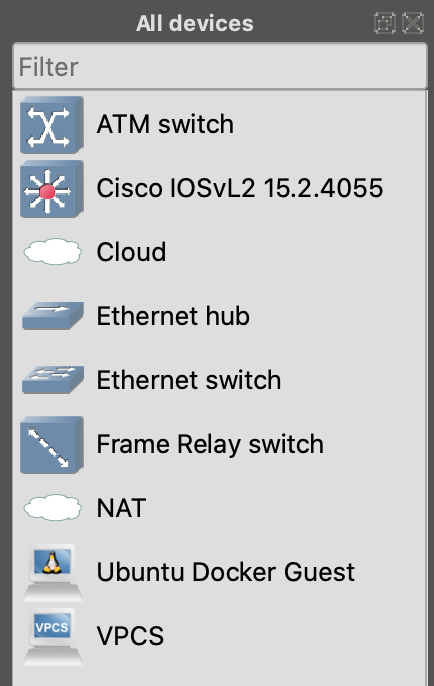
\includegraphics[width=.8\linewidth]{gns3-appliances-dock}
  \captionof{figure}{The appliances dock}
  \label{fig:gns3-appliances-dock}
\end{minipage}%
\begin{minipage}{.6\textwidth}
  \centering
  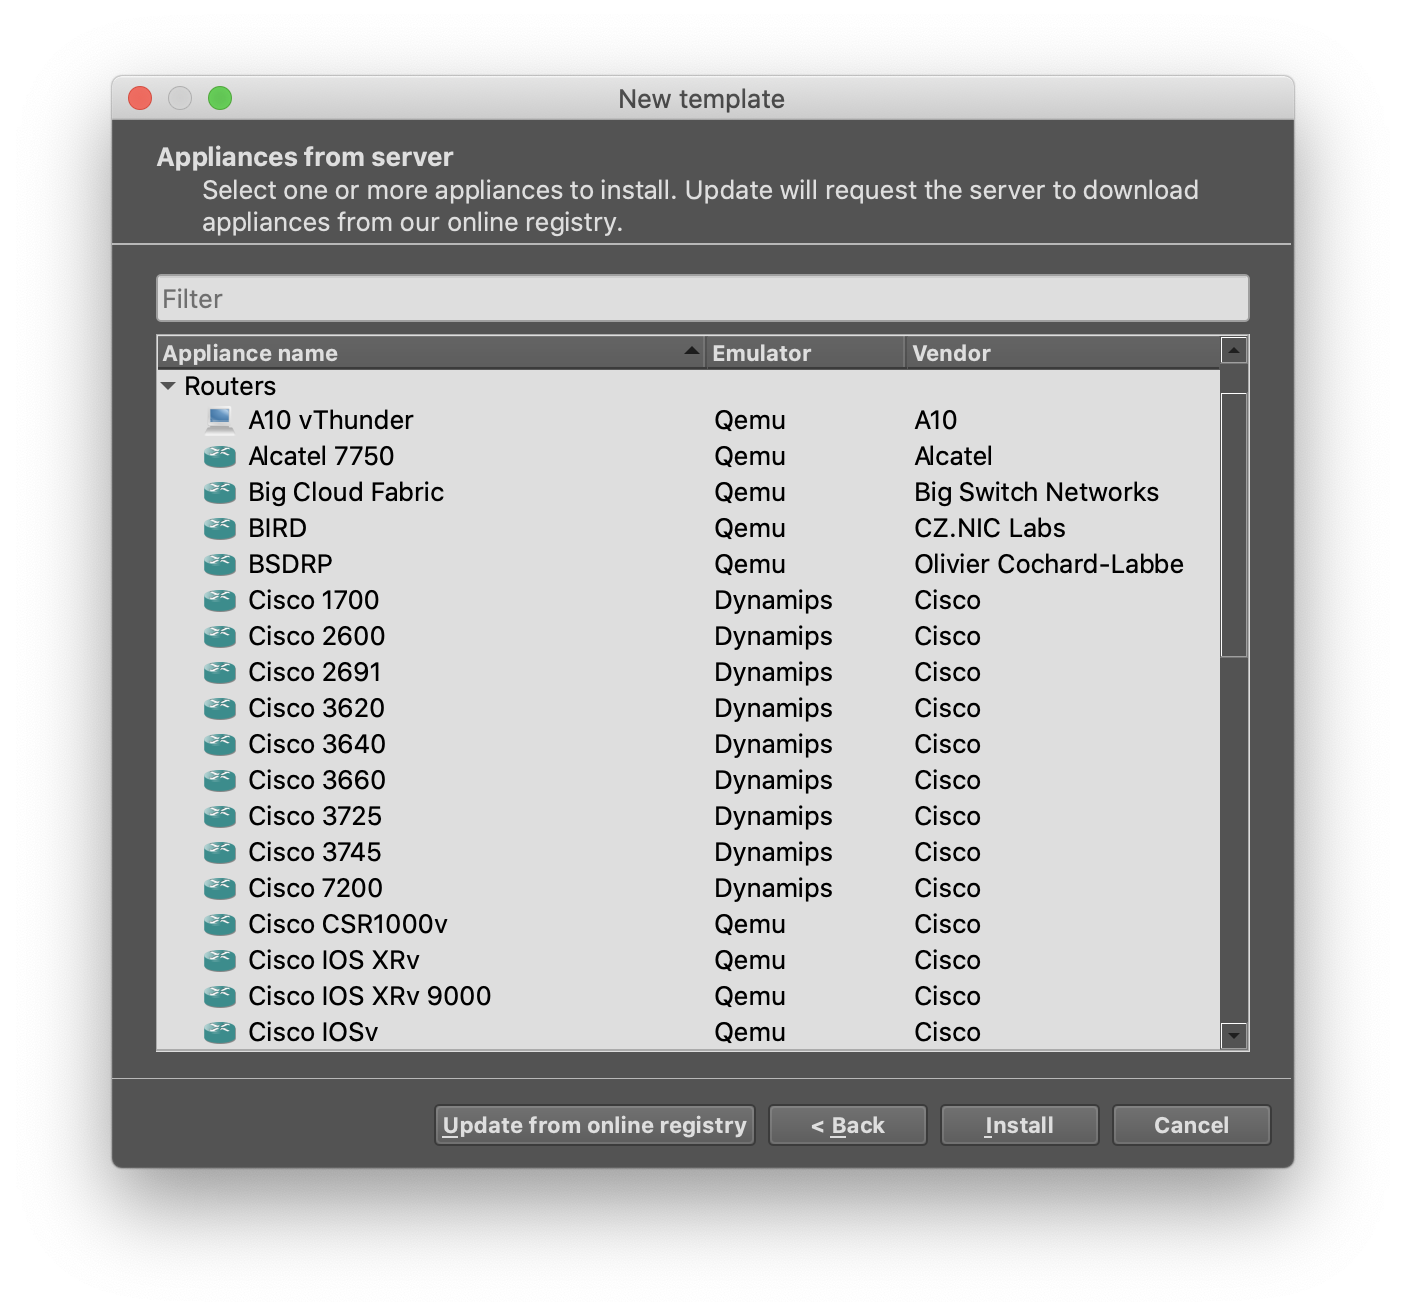
\includegraphics[width=.95\linewidth]{gns3-appliances-from-server-routers}
  \captionof{figure}{Some available router templates}
  \label{fig:gns3-appliances-from-server-routers}
\end{minipage}
\end{figure}


Deliberately, \emph{commercial} vendors of hardware, whose emulation is supported by GNS3, other than Cisco are excluded from this case-study for the following reasons:

\begin{enumerate}
  \item There isn't as near as many documentation and references in the literature, the web, or academic material for it as there is for Cisco.
  \item To narrow the scope of the investigation and this document, as the (again: commercial) network gear in laboratory used for the case study, FCT/NOVA's, is exclusively Cisco.
\end{enumerate}

Thus, this section is not intended to be exhaustive, or even less complete, in the sense of covering all the means GNS3 supplies out-of-the-box to emulate possible nodes in topologies.

\subsection{Dynamips and legacy Cisco routers}
\label{subsec:gns3dynamipslegacy}

GNS3 was initially built to leverage the Dynamips emulator~\cite{thebookofgns3}.
It consists of a pure hardware emulator for MIPS processors geared towards full-compatibility with a series of Cisco (now legacy) router hardware models, namely the 1700, 2600, 3600, 3700, and 7200 series. % TODO add 'MIPS' to gls
Not only it the emulator is able to execute MIPS machine-level instructions, it also is able to boot real, uncompressed images for the real hardware and provide virtual interfaces and slots for modules corresponding to those in the physical counterparts.

Dynamips does not support Cisco Catalyst layer-2 switches, only the aforementioned layer-3 modular routers.
All it offers for switching capabilities is, for some models, the ability to insert a module, called EtherSwitch, which provides 16 switched ports to the routers, and allows for \emph{some} experiments with the switching capabilities (VLANs, STP) to be made.
However,~\cite{thebookofgns3}, which has a lengthy reference on using Dynamips, its advantages and disadvantages is clear in stating that it isn't without its limitations, which comprehensively listed in this reference.

In a video published in the already mentioned semi-official GNS3 YouTube channel, the software's creator Jeremy Grossmann clearly states that Dynamips is not recommended for production these days, since, as will be seen later, more modern and maintainable solutions exist. At the same time, the GNS3 creator and lead developer also states that there are not plans to remove Dynamips support in upcoming versions~\cite{ytdynamipsvpcs}.

That is not say that, if no ``advanced'' features are intended, Dynamips, whose processes are extremely light compared to most of the alternatives (cf. <REFER TO THE PERFORMANCE PART WHEN READY>), isn't the right solution, in the user or institution has access to licensed legacy IOS images. % TODO add ref to the performance part

\subsection{QEMU and Cisco IOSv}
\label{subsec:gns3ciscoiosv}

Another way to have Cisco gear inside a topology is using Cisco IOSv images, provided by the vendor itself as part of having access to their proprietary Virtual Internet Routing Lab (VIRL)~\cite{ciscovirl}.
IOSv, which concretely are IOSvL2 and IOSvL3 (standing for layer-2 and layer-3, respectively) are described as ``an implementation of Cisco IOS running as a full virtual machine on a hypervisor''~\cite{ciscoiosvinfo}.

On GNS3 this is accomplished via QEMU, a free and open source, general purpose emulator.
In particular, the way GNS3 uses QEMU is not as an emulator, but as a wrapper for KVM~\cite{whatiskvm}, which ensures extremely good virtualized performance, though naturally limited to the resources of the hypervisor machine~:
\begin{displayquote}
Run KVM and Xen virtual machines with near native performance\footnote{\url{https://www.qemu.org}}
\end{displayquote}

When an appliance for IOSv is added to a GNS3 setup using the template, a virtual disk image is provided and uploaded to the compute node.
It is then used for spinning up VMs with virtual interfaces running the operating system provided in the image. % TODO make this an acr statement

\subsection{Guests and other appliances}
\label{subsec:gns3guestsappliances}

Bla bla bla.

\subsection{Links}
\label{subsec:links}

Yadda yadda yadda.

% TODO refer back to the ESXi running servers on clouds on virtualized machines and the need for enabling nested virtualization

% end of section gns3emulating
